\chapter{Template Fitting}
\label{ch:template}

The modified Quadratic Estimator (mQE) developed in the last chapter completely eliminates the thermal Sunyaev-Zel'dovich (SZ) bias by using a SZ free gradient map. 
Though SZ bias is removed in the mQE, SZ present in the lensing map induces extra variance in the reconstructed lensing convergence profile. 
Unlike the variance due to other sources (such as instrumental noise, uncorrelated foregrounds etc.,), SZ variance depends on the mass of the galaxy cluster.
The SZ variance scales roughly with the mass of the cluster as $M^{3.33}$.
For DES X SPTpol clusters which we used in the previous chapter, we downweighed the massive clusters to take the SZ variance into account. 
This didn't have much effect on the final SNR as we had only few massive clusters. 
However, with future low noise CMB surveys such as SPT-3G, CMB-S4, Simons Observatory etc.,\citep{bender18,cmbs4-sb1,so18} downweighing won't be an optimal solution.


This chapter is organised as follows: in \S\ref{sec_simulations} we explain the simulations used in this chapter. In \S\ref{sec_methods}, we describe the template fitting approach which will significantly reduce the SZ variance, followed by results in \S\ref{temp_fit_sec_results}. 
We forecast mass uncertainties for future experiments using our new method in ~\S\ref{forecasts} and then we finally conclude in \S\ref{temp_fit_conclusions}.

%I present template fitting approach which will significantly reduce the SZ variance in high mass cluster and/or low noise surveys. 
%I then discuss the effect of SZ variance and experimental variance as a function of experimental noise and cluster mass. 
\section{Simulations}
\label{sec_simulations}

We use simulations to validate our new method and also to forecast future experiments. 
%The simulations used here closely follow the ones described in chapter \ref{ch:MLE}.
 We create \mbox{$100^\prime \times 100^\prime$} unlensed Gaussian realizations of the \textit{Planck} 2015 \citep{planck15-13} best-fit lensed CMB power spectrum obtained from CAMB\footnote{\url{https://camb.info/}} \citep{lewis00} (as explained in chapter \ref{ch:MLE}).
These maps are then lensed by the cluster convergence profile (see \S\ref{sec_def_field}). 
We add simulated SZ emission (\S\ref{sec_tsz}) and then convolve the map by the assumed instrumental beam. 
We take the instrumental beam to be a Gaussian with a FWHM $=1^\prime.7$ at 95 GHz and $=1^\prime.0$ at 150 GHz. 
Finally, we add Gaussian realizations of white noise at the specified noise level. 
 


\subsection{thermal Sunyaev-Zel'dovich signal}
\label{sec_tsz}

Unless otherwise noted, we assume the SZ emission is described by a radially-symmetric  Arnaud profile \citep{arnaud10} expected for a cluster of the specified mass and redshift. 
We do test the robustness of this assumption in \S\ref{subsec:simsz} by using two sets of realistic SZ simulations from \citet{sehgal10} and \citet{takahashi17}. 
The SZ power in the \citep{sehgal10} simulations is scaled down by a factor of 1.75 to better match the measured SZ power in \cite{george15}; the \citet{takahashi17} simulations post-date the SZ measurements and are not rescaled. 
Extracting the appropriate SZ signal from these simulations requires selecting matching galaxy clusters, with a tradeoff between the number of matching clusters in the simulations and the fidelity of the match. 
 We randomly select halos which are within 5\% of the desired mass and $\pm 0.2$ of the desired redshift.

\section{Method}
\label{sec_methods}
In this section, we present a template fitting approach designed to reduce the SZ variance for massive galaxy clusters or for low noise surveys. 
We also discuss sources of uncertainties present in the CMB-cluster lensing analysis. 
\subsection{Template fitting to reduce the SZ variance}
\label{sec_sz_template_fitting}

An obvious way to eliminate the SZ variance is by using SZ-free maps for both the lensing and gradient maps. 
Of course this would undo the advantages of the modified QE for the instrumental noise in the lensing map. 
One can also reduce this extra variance by projecting out a model template for the SZ signal, and thereby reducing the total amount of SZ power in the lensing map. 
Given the impossibility in creating a `perfect' SZ template, the template fitting will not completely eliminate the SZ signal in the lensing map. 
However, template fitting can significantly reduce the SZ power in the lensing map, and thus reduce the SZ noise penalty on the lensing mass reconstruction. 



To be unbiased, we must fit the template to a CMB-subtracted map or account for the information loss from template projection in the normalization factor $A_l$ of Eqn.~\ref{mqe_convergence_eqn}. 
The latter tact (correcting $A_l$) might have advantages if one needed to suppress multiple kinds of cluster emission, e.g., dusty and radio galaxies in addition to the thermal SZ effect. 
Projecting a template from the Compton-$y$ map will not help these other cluster signals. 
However, we expect these other signals to be small compared to the SZ flux for massive galaxy clusters \footnote{While the statement is generally true, it is important to note that in some low redshift clusters radio emission from the AGN core can be much larger than the SZ signal and CIB may be significant for some high redshift clusters.}. %\pending{citations needed}. 
In this work, we take the first approach and fit the template to a Compton-$y$ map created from a linear combination of 95 and 150\,GHz maps. 
Effectively, we have used the different spectral dependence of the SZ and CMB to eliminate the CMB, and thus any correlation between the removed template and the lensing dipole in the CMB map. 

\begin{figure}[ht]
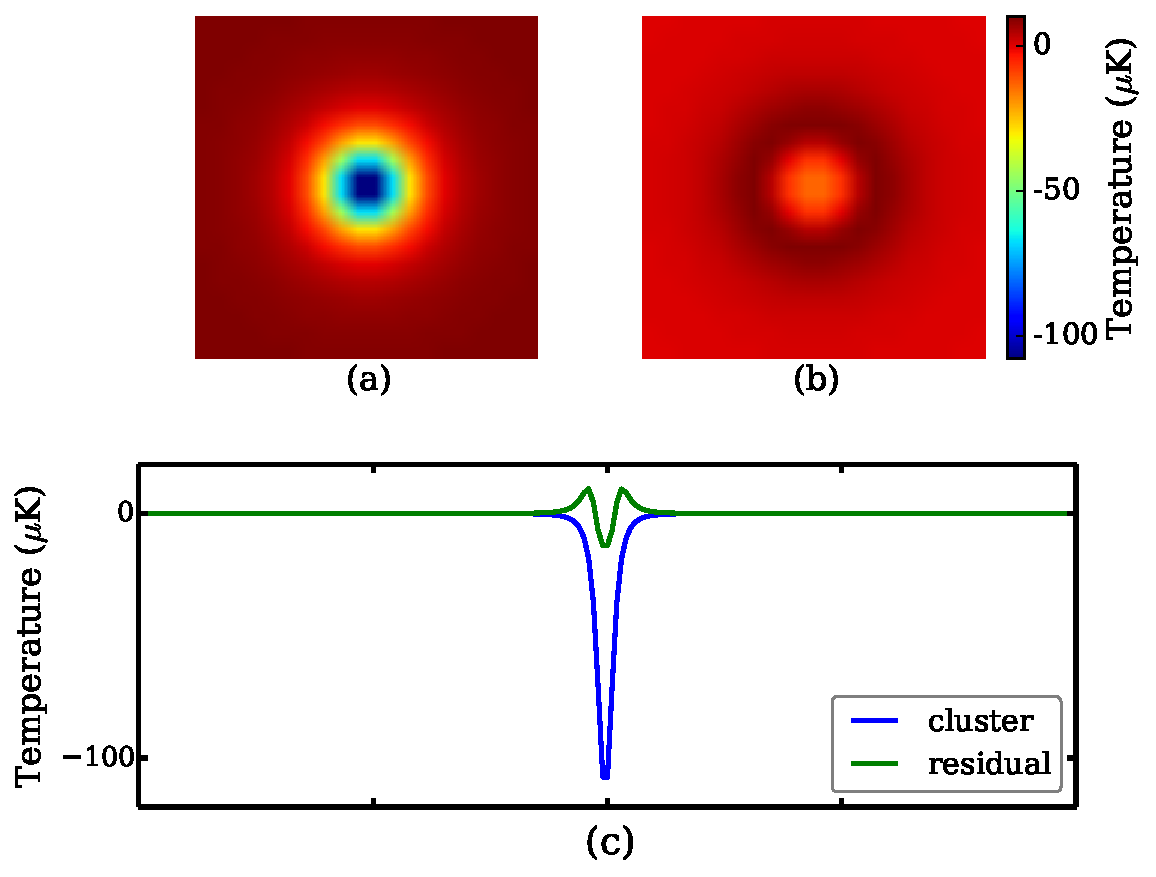
\includegraphics[width=\linewidth, keepaspectratio]{figs/template_fitting.pdf}
 \caption{Template fitting significantly reduces SZ power, even with an imperfect match between the template and true SZ signal. 
The top left panel (a) shows the expected Arnaud profile for a galaxy cluster of mass $\mvir = 5 \times \:\munits$ at z=0.7 after being smoothed by Gaussian beam with FWHM= 1\arcmin.7.
The top right panel (b) shows the residuals after subtracting the best-fit 2\arcmin.0 FWHM Gaussian (the amplitude is free, but the FWHM is fixed). 
The lower panel (c) shows one-dimensional slices through each panel: the solid blue line is a slice through the beam-convolved Arnaud profile of (a), and the dashed green line is a slice through the residual map in (b). 
 } 
\label{fig:residual}
\end{figure}
We choose to use a radially symmetric template at the fixed cluster location in this work. 
Unless otherwise noted, we assume the beam to be a Gaussian with FWHM = 1\arcmin{} at 150\, GHz and 1\arcmin.7 at 95\,GHz. 
As this beam size is significantly large compared to the actual size of clusters at $z>0.3$, clusters are approaching the effective point source limit where the specific details of their shape would not matter. 
Thus we choose to use a simple Gaussian template as the baseline template in this work. 
We also compare the results to template fitting with more physically motivated Arnaud profile \citep{arnaud10}, convolved by the experimental Gaussian beam.  
The residuals of removing a 2\arcmin.0 FWHM Gaussian from an Arnaud profile convolved by a 1\arcmin.7 beam are illustrated in Fig.~\ref{fig:residual}. 
As argued above, the Gaussian template significantly reduces the SZ signal despite the mismatch between the assumed profile and input SZ model. 
While there should be small variations in the typical size of the cluster's SZ emission with mass and redshift, we neglect these variations and fix the size of the templates based on the expected median mass and redshift of the sample. 
One could easily adjust the template based on individual cluster redshift for a minimal increase in complexity.



As SZ and CMB have different frequency dependence, we use linear combination of 95\, GHz and 150\, GHz channels to obtain Compton-$y$ maps.
%\begin{equation}
%T_{sz} = \frac{B_{90}}{B_{150}} T_{90} - T_{150} 
%\end{equation}
%Since the template will be applied to that lensing map that has been high pass filtered at $\ell > 2000$, we apply a matching high pass filter to the map used for fitting and the SZ model template. 
We then pull out a central $10\arcmin \times 10\arcmin$ cutout at the cluster location for fitting the template. 
Since the SZ emission is concentrated within a few arcminutes of the cluster center, there is little reason to fit over a larger area. 
We allow for two free parameters in the fitting: the overall amplitude of the template, and a constant DC background level. 
%Note that given the high-pass filter, we expect (and find) the DC term to be effectively zero. 
We include the DC term while fitting the template amplitude, however, we do not subtract DC level. 
Only the template is subtracted from the lensing map.



With template fitting included, the Fourier transforms of the two maps used by the quadratic estimator can be written down as:
\begin{eqnarray}
G_{\ell} &=& i\ell W^{G}_{\ell} T^{\rm SZ-free}_{\ell}\\
L_{\ell} &=& W^{L}_{\ell} \left(T_{\ell} - T_\ell^{\rm SZ-template}\right)
\end{eqnarray}
where, $G_{\ell}$ is the large-scale gradient map and $L_{\ell}$ is the lensing map. 
$W^{G}_{l}$ and $W^{L}_{l} $ are the Wiener filters to maximize the lensing signal \cite{hu07}. 
The mm-wave map is $T_{\ell}$ while the constructed SZ-free map is $T^{\rm SZ-free}_{\ell}$. 
Compared to the modified QE \citep{madhavacheril18,raghunathan18}, the new element is the $T_\ell^{\rm SZ-template}$ term representing the SZ template fit. 





\subsection{Sources of uncertainty in the CMB-Cluster Lensing Measurement}
\begin{figure}[htb]
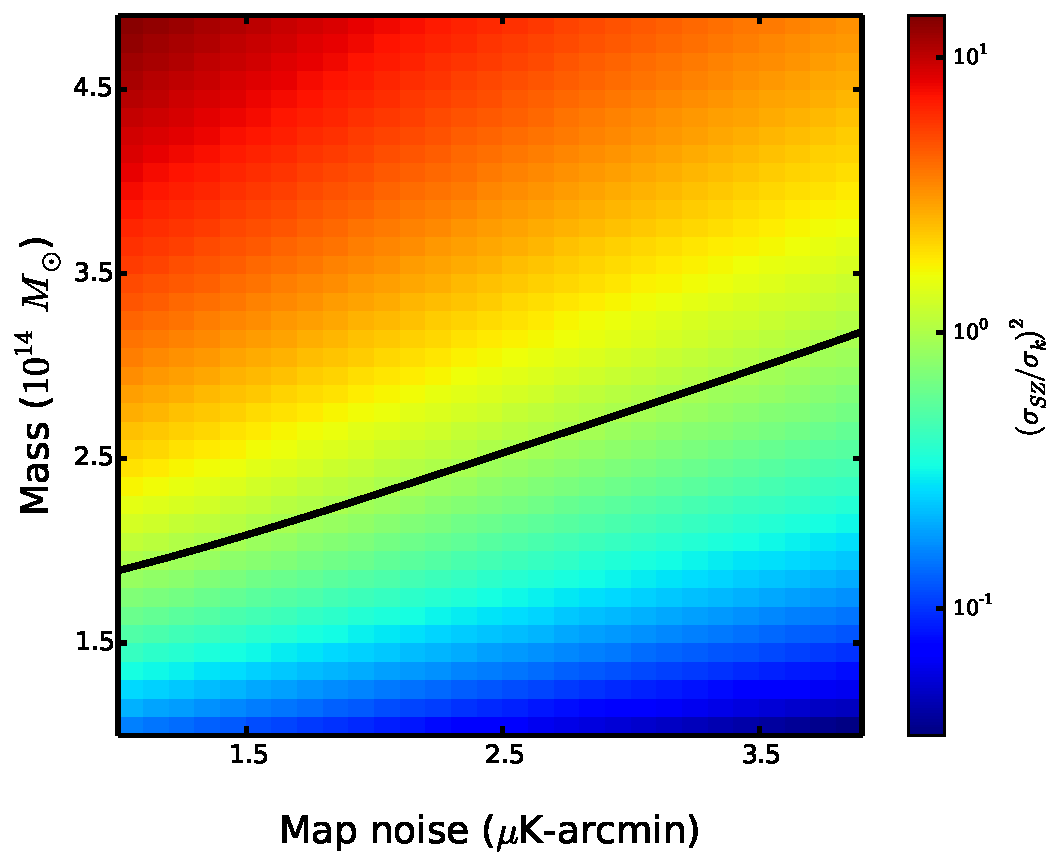
\includegraphics[width=\linewidth, keepaspectratio]{figs/contour_plot.pdf}
 \caption{
 Ratio of SZ variance over kappa variance as a function of cluster mass and experimental noise level. 
 As expected the ratio increases with mass for a given experimental noise level. 
 The black solid line represents the points where the SZ variance is equal to the non-SZ variance.
 %\pending{(SR 20190130: Can you make a contour plot here to also include the effect of map depth? That will be more intuitive and one can easily figure out the mass threshold for which this method will be effective for different surveys.)\\}
 %\pending{Axis labels and caption disagree: sigma/variance} 
 %\pending{\textbf{Plot change: Keep the dashed line for 'SZ variance'. Add several horizontal lines at eg 1uk-arcmin, 3-uk-arcmin, 10uk-arcmin. Y-axis will no longer be the ratio}}
  }
 \label{fig:variance}
\end{figure}

Template fitting is intended to reduce the SZ variance, however it will not suppress other sources of uncertainty such as instrumental noise, CMB sample variance and foreground emission. 
Thus it will be useful to look at the relative magnitudes of these two terms, the SZ variance ($\sigma_{SZ}^{2}$) and the non-SZ variance ($\sigma_{\kappa}^{2}$), when interpreting the performance of template fitting in the next section. 


The non-SZ variance or kappa variance depends on the survey parameters (i.e.~instrumental noise, and the degree to which foregrounds are cleaned) but is independent of the cluster properties. 
We estimate the non-SZ variance, $\sigma_{\kappa}^{2}$, using simulations of the CMB plus instrumental noise. 
Given the goal, we do not include the cluster's SZ emission.  
We apply the lensing pipeline to the simulated skies to estimate the convergence maps. 
We fit the convergence map  to determine  a mass, and take the scatter in these inferred masses over 1000 simulations to be $\sigma_{\kappa}$. 


In contrast, the SZ variance should increase with cluster mass, $M$, roughly as $\sigma_{sz}^2 \propto M^{10/3}$, while being independent of the survey parameters. 
We estimate the SZ variance using the same suite of simulations, however now adding the cluster's SZ emission to the lensing map. 
We continue using an SZ-free map for other leg of the QE, the large-scale gradient map. 
As before, we estimate the convergence maps, fit for masses and take the scatter in these inferred masses to estimate $\sigma_{SZ}^{2}$ + $\sigma_{\kappa}^{2}$.

We present the ratio of the SZ to non-SZ variances, $\sigma_{SZ}^{2}$/$\sigma_{\kappa}^{2}$, as a function of survey noise level and cluster mass in Fig.~\ref{fig:variance}.  
As expected, the ratio increases with mass at any given noise level. 
The black solid curve represents a ratio of unity when the SZ variance equals the non-SZ variance. 
We expect template fitting to significantly improve the mass uncertainties only for clusters above the black curve. 

\section{Results}
\label{temp_fit_sec_results}
%\pending{(SR 20190130: Have you tested the method for a slightly realistic tSZ profile like Sehgal?)} 

%In this section, first we quantify various sources of uncertanities in the final convergence maps as function of experimental noise level and cluster mass. 
%Later, we compare the performance of our new method for various templates. 
%We  then use some realistic SZ simulations to check the robustness of our method.
%Finally, we discuss the effects of miscentering on our lensing analysis.%three algorithms to estimate cluster masses:  
%(1) using an SZ-free map in the gradient leg and no SZ in the HPF leg of quadratic estimator 
%(2) using an SZ-free map only for the gradient leg of the QE, i.e. the modified QE, 
%and (3) improved version of the modified QE presented in this work, with an SZ-free map used for the gradient leg of the QE and projecting an SZ template out of the  HPF leg. 
%We rate the performance of each method,  as a function of both cluster mass and experimental noise levels,  by the estimated uncertainty on the recovered cluster mass. 



 \begin{figure}[thb]
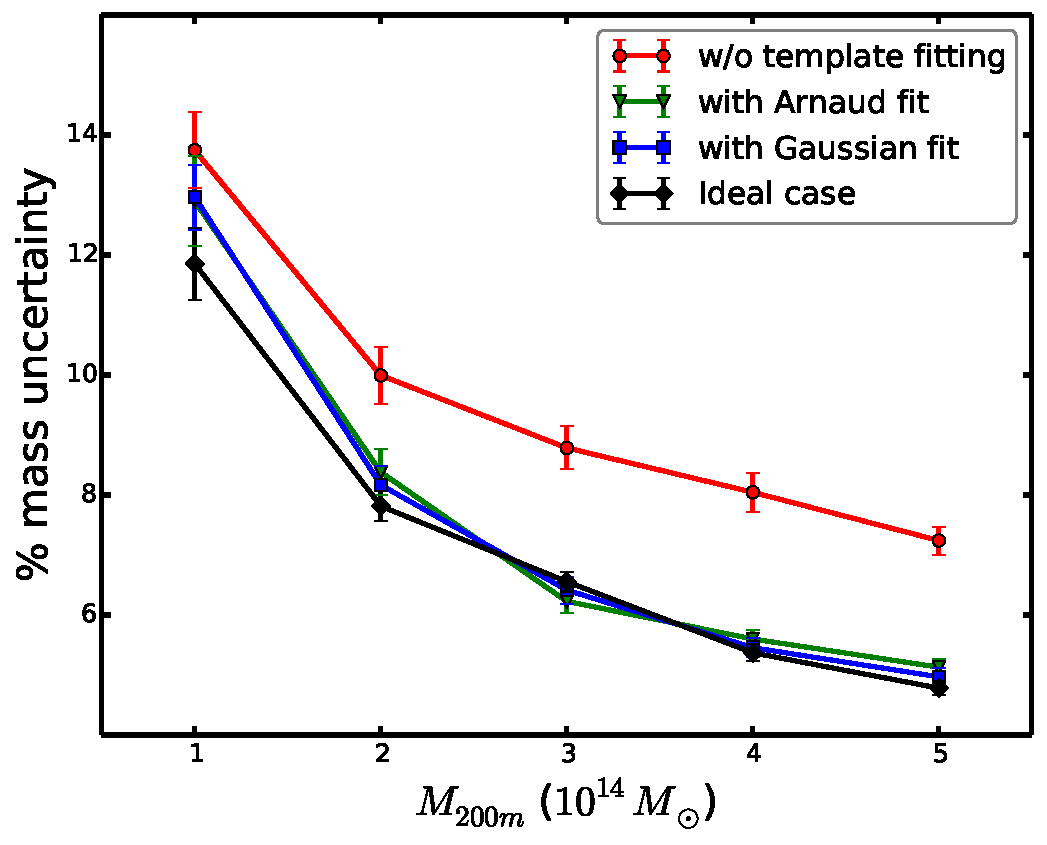
\includegraphics[width=\linewidth, keepaspectratio]{figs/uncen_vs_mass.pdf}
 \caption{
 Projecting out an SZ template from the second leg o the modified QE improves the performance for all masses considered. 
 Here we show the percentage mass uncertainties from three methods for a sample of 1000 clusters at a experimental noise level of 3\,\ukarcmin{}.
 All the curves use an SZ-free map for the gradient, but make different assumptions about the second, lensing filtered map. 
\label{fig:template_fitting}}
\end{figure}

As shown in Fig.~\ref{fig:template_fitting}, we find that template fitting leads to a significant improvement in the final mass uncertainties for CMB-cluster lensing. 
For high-mass clusters, template fitting does nearly as well as in the idealized (non-physical) limit of having no SZ emission. 
In this figure, we are assuming an SPT-3G like experiment with FWHM of 1$^\prime$ and 1.7$^\prime$ at 150\,GHz and  95\,GHz respectively and a survey noise level of 3\,\ukarcmin{}. 
We compare four algorithms to estimate cluster masses. 
In all cases we use a SZ-free gradient map (from a linear combination of 95 and 150\,GHz maps). 
%The tSZ emission injected in the high-pass filtered 150\,GHz map is based on an Arnaud profile. 
First, the red solid line shows the performance of the original modified QE without template fitting, where we have used SZ-free gradient map and 150GHz map with Arnaud SZ for the lensing map. 
%\sr{\sout{
%The second, black solid line shows the results for an idealized case, where we again use an SZ-free gradient map but use a 150\,GHz map without SZ for the lensing map. 
%While the latter assumption is unphysical since there will be SZ emission at 150\,GHz, it is useful as a  representation of the performance limit for perfect SZ subtraction. }
The second, black solid line shows the results for an idealized case, where we use a 150\,GHz map without SZ for the lensing map. 
While this assumption is unphysical since there will be SZ emission at 150\,GHz, it is useful as a representation of the performance limit for perfect SZ subtraction. 
Note that the relative performance improvement between the idealized and baseline case increases with mass as expected. 
For these survey parameters, the idealized case has 17\% smaller uncertainties than the baseline for clusters of mass $1\times 10^{14}\,M_{\odot}$ and 50\% smaller for cluster masses of $5\times 10^{14}\,M_{\odot}$. 
Template fitting recovers nearly all of this gain for high-mass clusters, as shown by the green triangles and blue squares (we have introduced an offset along mass axis for clarity). 
The two lines reflect different templates for subtraction. 
%\sr{\sout{The input simulated SZ signal is based on an Arnaud profile in both cases.}}
The green triangle shows the performance of projecting out an Arnaud SZ template from the lensing map. 
The blue square shows the results when using a Gaussian template instead, which is slightly mismatched to the assumed SZ signal. 
There is no practical performance difference between the two templates. 
For these assumed survey parameters, both templates are essentially indistinguishable from the idealized perfect SZ removal case at masses above $2\times 10^{14}\,M_{\odot}$. 
Template fitting does not do as well at lower masses. 
This can be understood by considering  the zero-mass limit -- where one tries to remove the SZ template from a map without SZ emission. 
The noisy estimate of the SZ template amplitude will set a non-zero, effective floor to the apparent SZ-like signal in this map. 
In the low-mass limit, SZ template removal will thus perform more poorly than the original estimator. 
The first signs of this transition can be seen in Fig.~\ref{fig:template_fitting} when comparing the performance at $\mvir = 2\times 10^{14}\,M_{\odot}$ to   $1\times 10^{14}\,M_{\odot}$.


 
 
%%%%%%%%%%%%%%%%%%%%%%%%%%%%%%%%%%%%%%%%%%%%%
%%%%%%%%%%%%%%%%%%%%%%%%%%%%%%%%%%%%%%%%%%%%%
%%%%%%%%%%%%%%%%%%%%%%%%%%%%%%%%%%%%%%%%%%%%%



%To calculate $\sigma_{\kappa}$, we use simulated tSZ free gradient and 150GHz maps, calculate the standard deviation within 10' from the center of the corresponding 'null' convergence maps. 
%The variance induced due to SZ is considerable for the clusters where ratio of $\sigma_{sz}/\sigma_{\kappa}$ is greater than 1. 
 
%\begin{figure}[h!]
%\includegraphics[width=\linewidth]{template_fitting_likelihood.png}
 %\caption{\pending{}}
 %\label{fig:boat1}
%\end{figure}
\iffalse{
\subsection{Miscentering}
\begin{figure}[ht]
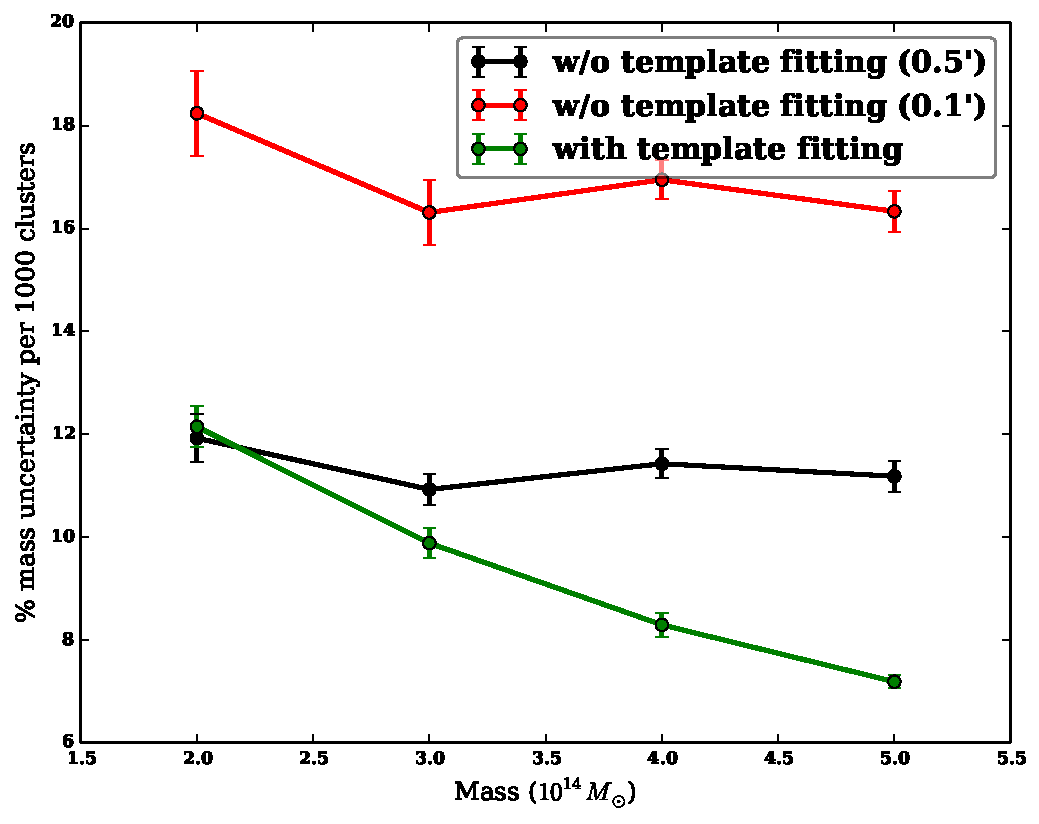
\includegraphics[width=\linewidth]{figs/miscentering_results.pdf}
 \caption{%Our new method is robust to realistic SZ simulations. 
The red and black solid curves show the performance of modified QE for the Sehgal and Takahashi simulations respectively. 
The dashed lines show the improvement in each case when template fitting is used to reduce the SZ variance in the lensing map. 
 \sr{ Change xlabel to $\mvir$}.
 }
\label{fig:realistic_sims_pos}
\end{figure}
Previous works have found a positional offset of 0.5$\arcmin$ between the SZ and X-ray centroid \citep{linden14} or location of the brightest central galaxy (BCG)\citep{song12b}.
Template fitting methods provides optimal results if cluster center is the SZ center.
While this is not a problem for SZ selected clusters as both cluster and SZ center coincide, however, this may be a concern for clusters selected via X-ray or optical surveys.

In order to check the performance of our new method in the presence of miscentering, we draw draw an offset between the true and nominal cluster position from a normal distribution, $N(0, \sigma^{2})$. 
We add the \citet{arnaud10} SZ profile at the offset location.
We perform the template fitting approach with additional fitting parameters for positional offsets.
The results are shown in Fig. \ref{{fig:realistic_sims_pos}}.
We 
 for two normal distributions $\sigma = 0.1\am\$.
As shown in the Fig. \ref{{fig:realistic_sims_pos}} template fitting approach will substantially reduce the SZ variance even in the case of miscentering. 

%It is important to note that in such cases we can't use high pass filtered map as the lensing induced ``dipol'' present in the HPF map biases our fitting to lower masses. %as the fitted positional offset will be.
%This bias can be removed by combining different frequency channels to remove CMB with slight decrement in SNR.
%Detailed analysis of positional offset effects are out of the scope this p
}\fi

\subsection{Robustness of template fitting method}
\label{subsec:simsz}
\begin{figure}[ht]
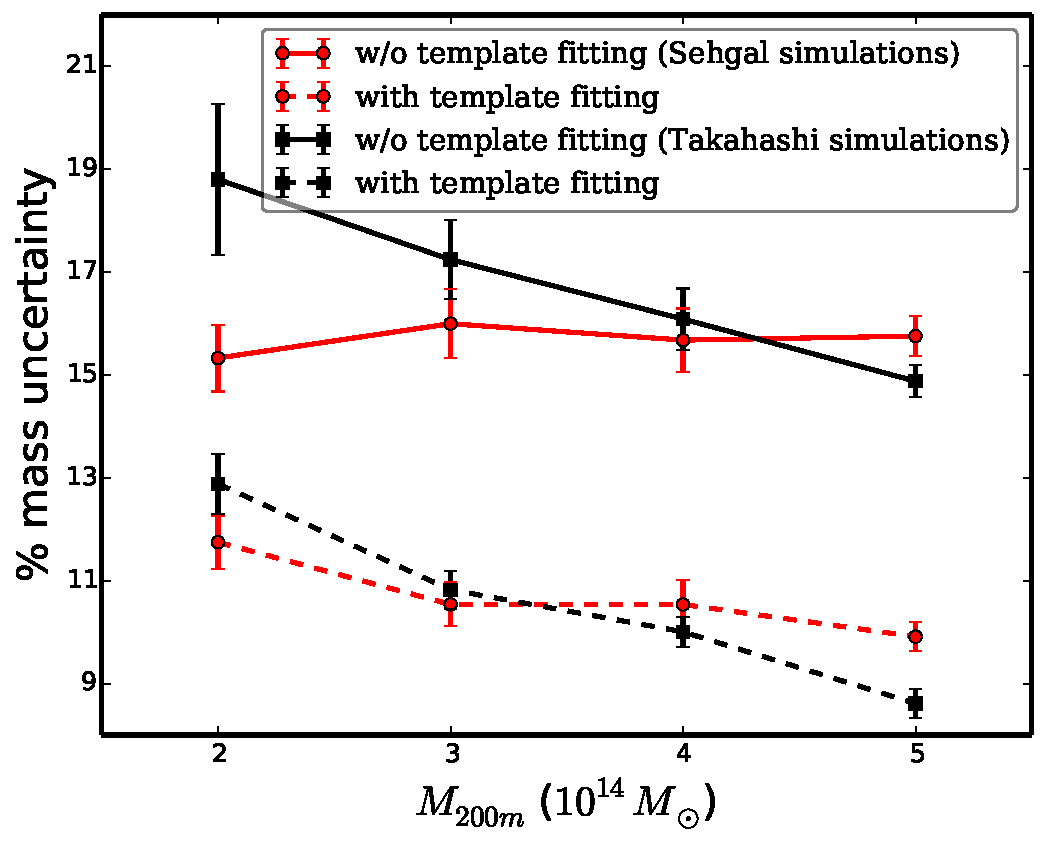
\includegraphics[width=\linewidth, keepaspectratio]{figs/Daisuke_Sehgal_results.pdf}
 \caption{
Our new method is robust to realistic SZ simulations. 
The red and black solid curves show the performance of modified QE for the Sehgal and Takahashi simulations respectively for a sample of 1000 clusters. 
The dashed lines show the improvement in each case when template fitting is used to reduce the SZ variance in the lensing map. 
The plotted uncertainties are for a stack of 1000 galaxy clusters of the quoted mass at $z=0.7$. 
 }
\label{fig:realistic_sims}
\end{figure}
As shown in the last section, the refinement to the modified QE improves the fractional mass uncertainties significantly (above a mass threshold that depends on the survey noise) for the symmetric Arnaud profile. 
However, the question remains as to whether this improvement will continue with the more complex real SZ emission of galaxy clusters along with any other haloes along the line-of-sight.
To test this, we turn to the SZ simulations of \citet{sehgal10, takahashi17}. 
As noted in \S\ref{sec_tsz}, we draw SZ maps from these sims centered at the locations of similarly massed haloes. 
The results for these sims are shown in Fig.~\ref{fig:realistic_sims} for Gaussian template fitting. 
We have tested using both the Gaussian and Arnaud template fitting, and have found no appreciable difference. 
Red lines are for the Sehgal simulations and black lines for the Takahashi simulations. 
The solid lines are without template fitting, while the dashed lines show the improvement from template fitting in each case. 
 The apparent flattening of the red curve is due the limited number of higher mass clusters in the Sehgal simulation. 
 %Sehgal simulations are sample variance limited especially at higher masses.
 In this case of realistic SZ signals, however, we note that the performance is not equivalent to the idealized case presented as black solid curve in Fig. \ref{fig:template_fitting}. 
This is due to the residual SZ signals in the map coming from the template mismatch, for example fitting a spherically symmetric template does not account for the cluster asphericity \footnote{By allowing more morphological freedom to the template might reduce this variance.}. In addition, the SZ signal from adjacent halos which we do not attempt to remove will also result in additional variance.
 



%\subsection{Miscentering}
%Previous works have found a positional offset of 0.5$\arcmin$ between the SZ and X-ray centroid \citep{linden14} or location of the brightest central galaxy (BCG)\citep{song12b}.
%Template fitting methods provides optimal results if cluster center is the SZ center.
%While this is not a problem for SZ selected clusters as both cluster and SZ center coincide, however, this may be a concern for clusters selected via X-ray or optical surveys.
%In such cases our new method will be optimal if we have additional fitting parameters for positional offsets.
%It is important to note that in such cases we can't use high pass filtered map to fit template as the lensing induced ``dipole" present in the HPF map biases our fitting to lower masses. %as the fitted positional offset will be.
%This bias can be removed by combining different frequency channels to remove CMB with slight decrement in SNR.
%Detailed analysis of positional offset effects are out of the scope this p


\section{Forecasts}
\label{forecasts}

We now consider the impact of this method on the performance of upcoming CMB surveys, SPT-3G \citep{bender18}, SO \citep{so18} and CMB-S4 \citep{cmbs4-sb1}. 
For the latter two experiments, we only consider the large-aperture telescopes (LAT) with an experimental beam of $\theta_{\rm FWHM} = 1.^{\prime}4$ at 150 GHz and covering 40\% of the sky (see also Table \ref{table_forecast_setup}). 
For SPT-3G, we assume a survey area of 1500\,\sqdeg{} and an experimental beam of $\theta_{\rm FWHM} = 1.^{\prime}2$ at 150 GHz. 
We create a single cluster catalog realization for each experiment based on the noise levels at 150\,GHz. 
Note that for simplicity, we make no attempt to use frequency information to remove other temperature foreground signals such as the the CIB, nor to improve the noise level on the Compton-y map. 
These assumptions are likely to mean that the simulated cluster list is conservative since we are not taking advantage of the multiple frequency bands in each of these experiments. 

%The simulated 150\,GHz maps used for cluster finding include the primary CMB anisotropy, Gaussian foregrounds uncorrelated with the clusters, cluster SZ emission modelled using Arnaud profile, and the respective white noise levels as given in Table \ref{table_forecast_setup}.
%Next, we use the publicly available Halo Mass Function calculator \citep{murray13} to obtain the halo counts $d^{2}N/(dz\ d{\rm log}M$) per unit redshift ($\Delta z = 0.1$) and mass ($\Delta {\rm log} M = 14.05$) bin. %https://arxiv.org/abs/1306.6721
%Using the results from the above simulations, we get the number of clusters that will be detected above $\snr\ge 5$ by the three experiments. 
%This detection $\snr$ threshold should be conservative as well (the sample purity should be close to 1). 
%We estimate that SPT-3G, SO and CMB-S4 will detect respectively approximately 2,400, 27,000 and 75,000 clusters.


The three simulated cluster sample and assumed experimental parameters are passed through the cluster-lensing pipeline to estimate the mass uncertainty from CMB-cluster lensing on each stacked sample. 
 For forecasts we picks SZ profiles from \cite{takahashi17} simulations and as mentioned before we randomly pick all the halos which fall within 5\% of the desired mass and $\pm$0.2 of the desired redshift.
The results are given in Table \ref{table_forecast_setup}. 
We find that template fitting can reduce the percentage mass uncertainty for SPT-3G, SO and CMB-S4 by 28\%, 25\% and 30\% respectively.% 37\%, and 30\% for SPT-3G, SO, and CMB-S4 respectively. 
%The drop-off in the improvement for CMB-S4 here is because CMB-S4 is expected to detect lower mass clusters, where the SZ variance is less important relative to the CMB and instrumental noise variance. 
%When restricted to massive clusters at $M > 4 \times 10^{14}\msol$, we see an approximately 40\% improvement in detection significance for all three experiments. \tbd{confirm this}. 


\begin{table}
\caption{Forecasted mass uncertainties for SPT-3G, SO and CMB-S4  with the modified QE before and after removing the estimated SZ template.}
\footnotesize{
\centering
%\begin{tabular}{| C{1.5cm} | C{1.2cm}|  C{0.8cm} | C{1cm} | C{1cm} | C{1cm}  |}
\begin{tabular}{| c | c |  c | c | c  |}
\hline
% \multirow{2}{*}{Experiment} &  \multirow{2}{*}{$\Delta_{T}\ [\mu K^{\prime}]$} & \multirow{2}{*}{$f_{\rm sky}$} & \multirow{2}{*}{N$_{\rm clus}$} & \multicolumn{2}{c|}{$\Delta M/M$}\\
 \multirow{2}{*}{Exp.} &  \multirow{2}{*}{$\Delta_{T}\ [\mu K^{\prime}]$} & \multirow{3}{*}{N$_{\rm clus}$} & \multicolumn{2}{c|}{$\Delta M/M\ [\%]$}\\
\cline{4-5}
 & & & No template fitting & With template fitting\\\hline
SPT-3G & 2.2 & 2,400 &11.10& 8.00 \\\hline
 SO-LAT & 6.0 & 27,000 &2.82 &2.12 \\\hline
CMB-S4 & 1.73 & 75,000 &1.92 & 1.33\\\hline

\end{tabular}
}
\label{table_forecast_setup}
\end{table}


%%%%%%%%%%%%%%%%%%%%%%%%%%%%%%%%%%%%%%%%%%%%%
%%%%%%%%%%%%%%%%%%%%%%%%%%%%%%%%%%%%%%%%%%%%%
%%%%%%%%%%%%%%%%%%%%%%%%%%%%%%%%%%%%%%%%%%%%%
\section{Discussion and Conclusion}
\label{temp_fit_conclusions}

We have presented an improved version of the QE to estimate galaxy cluster masses through CMB lensing. 
By projecting out an SZ template from the lensing map of the QE, the algorithm substantially reduces the variance due to a cluster's own SZ emission. 
The SZ variance can be significant fraction of the total variance for high-mass clusters or low-noise surveys. 
Note that in the opposite limit of low masses or high noise (i.e. when the SZ variance is negligible), this template fitting may slightly reduce the overall S/N. 

%\sr{Keeping this paragraph depends on the sigma for SZ sims...}.
While the performance of the template fitting does depend on the fidelity with which the template accurately represents the true SZ signal, these variations do not seem to be a significant issue. 
In part this is because upcoming CMB experiments will not have sufficient angular resolution to resolve most of the structure in the SZ emission; the instrumental beam at 150\,GHz for a 6-meter telescope is slightly larger than a typical high-redshift cluster. 
%\sr{Check what happens to fig4: \sout{We get similar results as far as the final mass uncertainties for two independent sets of SZ simulations} %\citep{sehgal10, takahashi17}}. 
For mock SZ signals modeled using Arnaud profile, we find that the template removal approach reduces all of the additional variance due to the SZ signal. 
The improvement is not 100\% for realistic SZ signals \citep{sehgal10, takahashi17} because of the SZ emission from the adjacent haloes along the line-of-sight that we do not attempt to remove. 

The method presented in this work is not limited to the cluster lensing. 
For example, \citet{madhavacheril18} demonstrated that the modified QE can also be employed to CMB lensing in general. 
However, as shown here the thermal SZ signal from clusters detected at high \snr{} adds extra variance in the reconstructed lensing maps. 
By using template fitting approach we reduced the variance significantly. 
In future CMB lensing work, we can use the template fitting approach instead of masking the massive galaxy clusters. 
%While the thermal SZ signal does not bias the lensing reconstruction, the extra variance introduces a bias in the lensing auto-spectrum. 
%Write more ....}

CMB-cluster lensing will be a key tool for galaxy cluster cosmology at high redshifts, while also providing a cross-check of optical weak lensing mass estimates at lower redshifts. 
%For future CMB surveys such as CMB-S4 and SO we can improve the mass uncertainty by 30\% and 37\% respectively.
For future surveys like CMB-S4 and Simons Observatory and for clusters above masses of $4\times 10^{14}\,\msol$, we find that template fitting yields a factor of 1.4 reduction in the mass uncertainties. 
These results will help us in the quest to understand dark energy and the accelerating expansion of the Universe.


\iffalse{
\subsection*{Acknowledgements}
We thank Eric Baxter, Federico Bianchini, Thomas Crawford, Nikhel Gupta, Daisuke Nagai, and W. L. Kimmy Wu for useful discussions regarding this project.

SP acknowledges support from MIPP, Laby Travel Bursary, and Melbourne International Engagement Award. 
SR acknowledges the support from NSF grants AST-1716965 and CSSI-1835865.
The work at Melbourne is supported by the Australian Research Council's Discovery Projects scheme (DP150103208).
We thank the high performance computation center at the University of Melbourne for providing access to the cluster \texttt{spartan.unimelb.edu.au}.
We acknowledge the use of \texttt{CAMB} \citep{lewis02b} and \texttt{HEALPIX} \citep{gorski05} routines. 
This research used resources of the National Energy Research Scientific Computing Center (NERSC), a DOE Office of Science User Facility supported by the Office of Science of the U.S. Department of Energy under Contract No. DE-AC02-05CH11231. 
 %This work is performed in the context of the South Pole Telescope scientific program. 
 %SPT is supported by the National Science Foundation through grant PLR-1248097.


\section{Results}
\subsection{Sources of uncertainty in the CMB-Cluster Lensing Measurement}
\begin{figure}[htb]
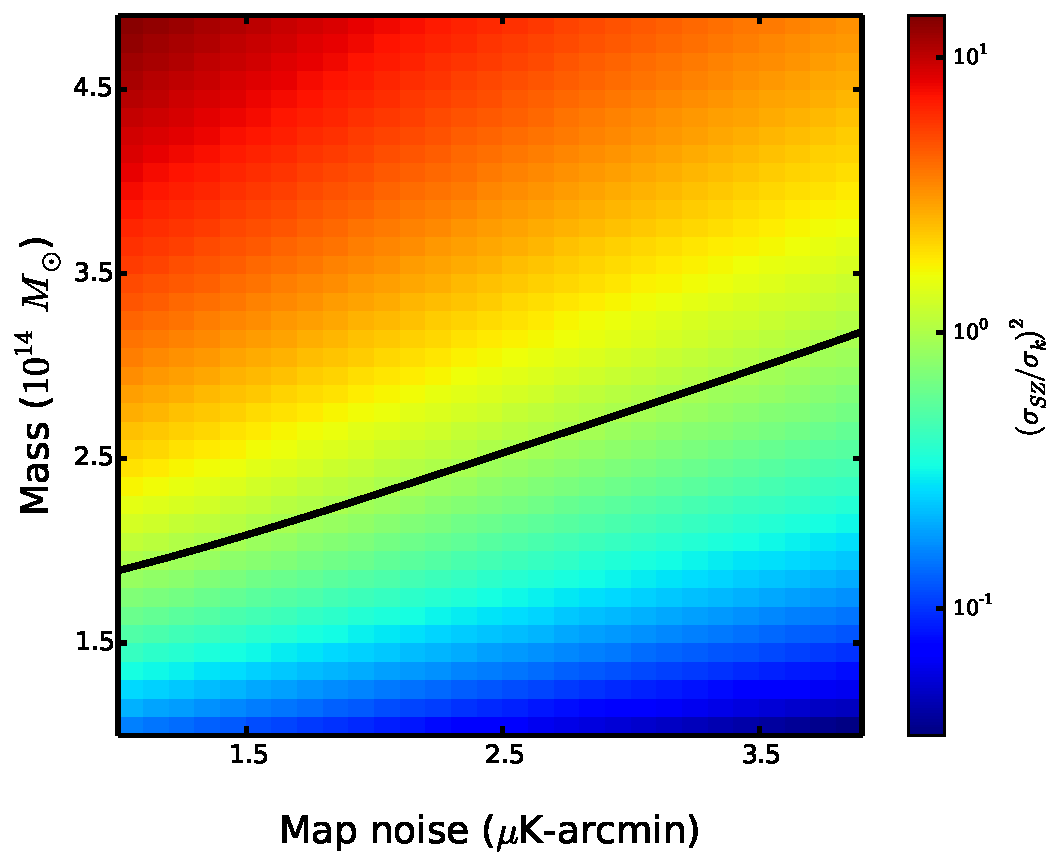
\includegraphics[width=\linewidth]{figs/contour_plot.pdf}
\vspace{-12pt}
 \caption{
 Ratio of SZ variance over kappa variance as a function of cluster mass and experimental noise level. 
 As expected the ratio increases with mass for a given experimental noise level. 
 The black solid line represents the points where the ratio SZ variance is equal to that of experimental noise.
 %\pending{(SR 20190130: Can you make a contour plot here to also include the effect of map depth? That will be more intuitive and one can easily figure out the mass threshold for which this method will be effective for different surveys.)\\}
 %\pending{Axis labels and caption disagree: sigma/variance} 
 %\pending{\textbf{Plot change: Keep the dashed line for 'SZ variance'. Add several horizontal lines at eg 1uk-arcmin, 3-uk-arcmin, 10uk-arcmin. Y-axis will no longer be the ratio}}
  }
 \label{fig:variance}
\end{figure}

Template fitting is intended to reduce the SZ variance, however it will do nothing for other sources of uncertainty such as instrumental noice, CMB sample variance and foreground emission (if not cleaned). 
Thus it will be useful to look at the relative magnitudes of these two terms, the SZ variance ($\sigma_{SZ}^{2}$) and the non-SZ variance ($\sigma_{\kappa}^{2}$), when interpreting the performance of template fitting in the next section.
The non-SZ variance, $\sigma_{\kappa}^{2}$, depends on the survey parameters (i.e.~instrumental noise, and the degree to which foregrounds are cleaned) but is independent of the cluster properties. 
We estimate $\sigma_{\kappa}^{2}$ following the approach in \citet{raghunathan18}. 
Briefly, we generate simulated CMB skies and add instrumental noise. 
We do not include the cluster's SZ emission or gravitational lensing signal since the goal is to estimate the other noise terms. 
We apply the lensing pipeline to the simulated skies to estimate the convergence maps. 
We fit the convergence map  to determine  a mass, and take the scatter in these inferred masses over 1000 simulations to be $\sigma_{\kappa}$. 
\tbd{think I've made this inaccurate. need to fix/explain better}

In contrast, the SZ variance should increase with cluster mass, $M$, roughly as $\sigma_{sz}^2 \propto M^{10/3}$, while being independent of the survey parameters. 
We estimate the SZ variance using the same suite as simulations, however now adding the cluster's SZ emission to the lensing lensing map. 
We continue using an SZ-free map for other leg of the QE, the large-scale gradient map. 
As before, we estimate the convergence maps, fit for masses and take the scatter in these inferred masses to estimate $\sigma_{SZ}^{2}$ + $\sigma_{\kappa}^{2}$.

We present the ratio of the SZ to non-SZ variances, $\sigma_{SZ}^{2}$/$\sigma_{\kappa}^{2}$, as a function of survey noise level and cluster mass in Fig.\ref{fig:variance}.  
As expected, the ratio increases with mass at any given noise level. 
The black solid curve represents a ratio of unity when the SZ variance equals the non-SZ variance. 
We expect template fitting to significantly improve the mass uncertainties only for clusters above the black curve. 

\section{Results}
\label{sec_results}
%\pending{(SR 20190130: Have you tested the method for a slightly realistic tSZ profile like Sehgal?)} 

%In this section, first we quantify various sources of uncertanities in the final convergence maps as function of experimental noise level and cluster mass. 
%Later, we compare the performance of our new method for various templates. 
%We  then use some realistic SZ simulations to check the robustness of our method.
%Finally, we discuss the effects of miscentering on our lensing analysis.%three algorithms to estimate cluster masses:  
%(1) using an SZ-free map in the gradient leg and no SZ in the HPF leg of quadratic estimator 
%(2) using an SZ-free map only for the gradient leg of the QE, i.e. the modified QE, 
%and (3) improved version of the modified QE presented in this work, with an SZ-free map used for the gradient leg of the QE and projecting an SZ template out of the  HPF leg. 
%We rate the performance of each method,  as a function of both cluster mass and experimental noise levels,  by the estimated uncertainty on the recovered cluster mass. 

As shown in Fig.~\ref{fig:template_fitting}, we find that template fitting leads to a significant improvement in the final mass uncertainties for CMB-cluster lensing. 
For high-mass clusters, template fitting does nearly as well as in the idealized (non-physical) limit of having no SZ emission. 
In this figure, we are assuming an SPT-3G like experiment with FWHM=1$^\prime$ at 150\,GHz and a survey noise level of 3\,\ukarcmin{}. 
We compare four algorithms to estimate cluster masses.  
First, the red solid line shows the performance of the original modified QE without template fitting. 
This uses  an SZ-free gradient map 
(from a linear combination of 95 and 150\,GHz maps) and use a 150\,GHz map with SZ emission for the two legs of the QE. 
The second, black dotted line shows the results for an idealized case, where we again use an SZ-free gradient map but use a 150\,GHz map without SZ for the lensing map. 
Obviously the latter assumption is unphysical since there will be SZ emission at 150\,GHz, but it shows the limit for how well perfect SZ subtraction might perform. 
Note that the relative performance improvement between the idealized and baseline cases increases with mass as expected. 
For these survey parameters, the idealized case has 17\% smaller uncertainties than the baseline for clusters of mass $1\times 10^14\,M_{\odot}$ and 50\% smaller for cluster masses of $5\times 10^14\,M_{\odot}$. 
Template fitting recovers nearly all of this gain for high-mass clusters. 


modified QE uncertainties 


(leaving out SZ)

for the gradient map and using 


no SZ in the lensing map of the QE. 
(2) using an SZ-free map only for the gradient leg of the QE, i.e. the modified QE, 
 and (3) improved version of the modified QE presented in this work, with an SZ-free map used for the gradient leg of the QE and projecting an SZ template out of the  HPF leg.
 
 \subsection{Performance comparision} 
Here we compare three algorithms to estimate cluster masses:  
(1) using an SZ-free map in the gradient leg and no SZ in the HPF leg of quadratic estimator
(2) using an SZ-free map only for the gradient leg of the QE, i.e. the modified QE, 
 and (3) improved version of the modified QE presented in this work, with an SZ-free map used for the gradient leg of the QE and projecting an SZ template out of the  HPF leg. 


The performance of the three algorithms are shown in Fig. ~\ref{fig:template_fitting} as a function of cluster mass for an SPT-3G like experiment.
 All the curves show the percentage mass uncertanity for a sample 1000 clusters. 
Black curve represents an ideal case - SZ free gradient and no SZ in the second leg.
Though not realistic, it gives lower bound we can achieve with template fitting. 
On the other hand, red curve gives the upper bound with SZ-free gradient and Arnaud SZ profile in the second leg.
Blue and green curves show the improvement that can be achieved using our new method. 
For the blue and green curves, SZ signal present in the second leg is reduced by using Gaussian and Arnaud templates respectively.


As can be seen, both Arnaud and Gaussian template fitting perform equally well.
 This is unsurprising given that the angular size of the clusters is somewhat smaller than the instrumental beams; the beam-convolved signal is close to a Gaussian. 
While ideally template fitting approach should outperform modified QE at all mass scales, this is not the case in reality.
At low cluster masses, experimental noise level dominates over SZ noise.
 In such cases the template fitting would be poor and our new approach achieves a minimal improvement over modified QE. 
%At low cluster masses our new method is consistent with modified QE as experimental noise dominates. 
 On the other hand, at higher masses SZ variance is dominant source of uncertainty where the performance of our new method is considerable with the ideal case. %\sr{This definitely requires more explanation.} 
 \pending{The improvement which we obtain over the modified QE depends on the mass of the cluster and the experimental noise level.
 While ideally template fitting approach should outperform modified QE at mass scales, this is not the case in reality.}
 \begin{figure}[htb]
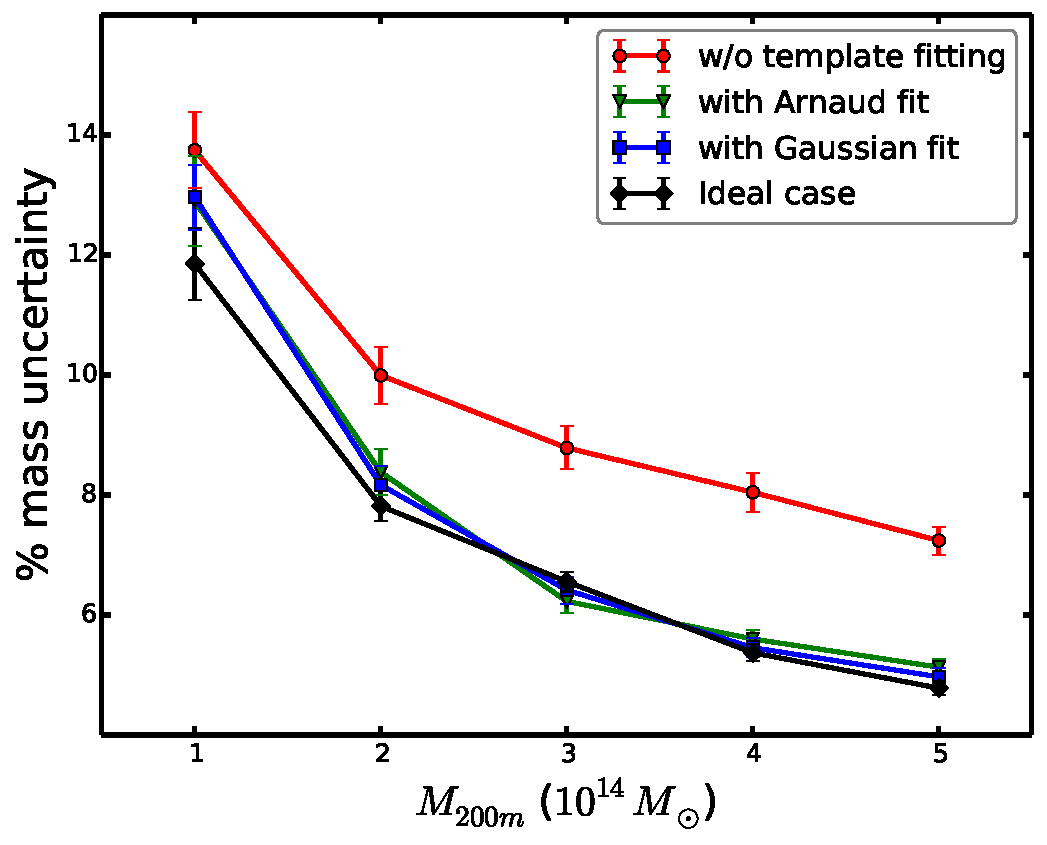
\includegraphics[width=\linewidth]{figs/uncen_vs_mass.pdf}
 \caption{
 Projecting out an SZ template from the second leg o the modified QE improves the performance for all masses considered. 
 Here we show the percentage mass uncertainties from three methods for a sample of 1000 clusters at a experimental noise level of 3\,\ukarcmin{}.
 All the curves use an SZ-free map for the gradient, but make different assumptions about the second, lensing map. 
 %In the ideal case (red), the HPF map assumes 150\,GHz map noise levels with zero SZ signal -- a physically unrealistic option that is included to show the lower bound to how well a method to deal with the SZ signal might perform. 
 %At the other extreme, the green curve shows the results when a raw 150\,GHz map is used for the HPF leg, i.e.~it includes the full effects of SZ variance and sets the upper bound on the performance of methods to remove the SZ variance. 
 %The uncertainties for the simple template fitting method are shown by the black line. 
 %As expected, it falls between the two extremes. 
 %For low-mass clusters \pending{(M = 2e14) }, the template fitting method only marginally improves the results -- reducing the already small SZ variance is balanced against the information loss from the mode projection. 
%At higher masses where the SZ variance is dominant since it scales as $M^{5/3}$, the template fitting method does extremely well compared to using an 150\,GHz map (the green curve). 
 \sr{Replace ``mQE' to w/o template fitting. They are all mQE. Change xlabel to $\mvir$. Change line styles to match text}.
 }
\label{fig:template_fitting}
\end{figure}
\subsection{Robustness of template fitting method}
\label{subsec:simsz}
As seen in the Fig.~\ref{fig:template_fitting} our refinement for modified QE improves the fractional mass uncertanties sginificantly for all the masses considered.
 However, the realistic SZ may not be a radially symmetric as Arnaud profile predicts.
So, in order to check the robustness of our new method we used realistic SZ simulations from Sehgal et al \cite{sehgal10} and Takahashi et al \cite{takahashi17}, the results of which are show in Fig.~\ref{fig:realistic_sims}. 
We have only considered Gaussian fitting for the realistic simulations as there is no difference in the performance of both templates.  
The red and black curves in the figure are the results of modified QE for Sehgal and Daisuke sims and the corresponding dashed curves show the improvements we obtain after subtracting Gaussian template from the second leg of modified QE.
 The apparent flattening of the red curve is due the limited sample variance of Sehgal simulation at higher masses.
 %Sehgal simulations are sample variance limited especially at higher masses.

\begin{figure}[htb]
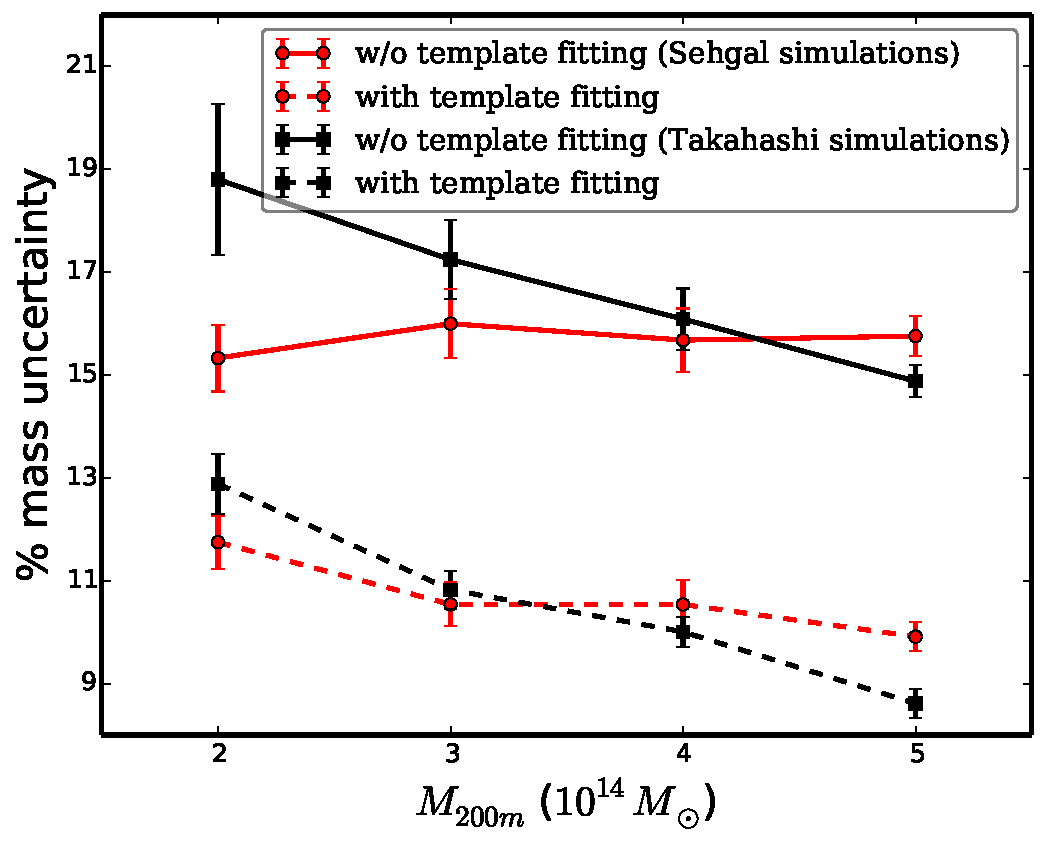
\includegraphics[width=\linewidth]{figs/Daisuke_Sehgal_results.pdf}
 \caption{
Our new method is robust to realistic SZ simulations. 
The red and black solid curves show the performance of modified QE for the Sehgal and Takahashi simulations respectively. 
The dashed lines show the improvement in each case when template fitting is used to reduce the SZ variance in the lensing map. 
 \sr{ Change xlabel to $\mvir$}.
 }
\label{fig:realistic_sims}
\end{figure}

\subsection{Miscentering}
Previous works have found a positional offset of 0.5$\arcmin$ between the SZ and X-ray centroid \citep{linden14} or location of the brightest central galaxy (BCG)\citep{song12b}.
Template fitting methods provides optimal results if cluster center is the SZ center.
While this is not a problem for SZ selected clusters as both cluster and SZ center coincide, however, this may be a concern for clusters selected via X-ray or optical surveys.
In such cases our new method will be optimal if we have additional fitting parameters for positional offsets.
It is important to note that in such cases we can't use high pass filtered map as the lensing induced ``dipole" present in the HPF map biases our fitting to lower masses. %as the fitted positional offset will be.
This bias can be removed by combining different frequency channels to remove CMB with slight decrement in SNR.
%Detailed analysis of positional offset effects are out of the scope this p
\begin{figure}[htb]
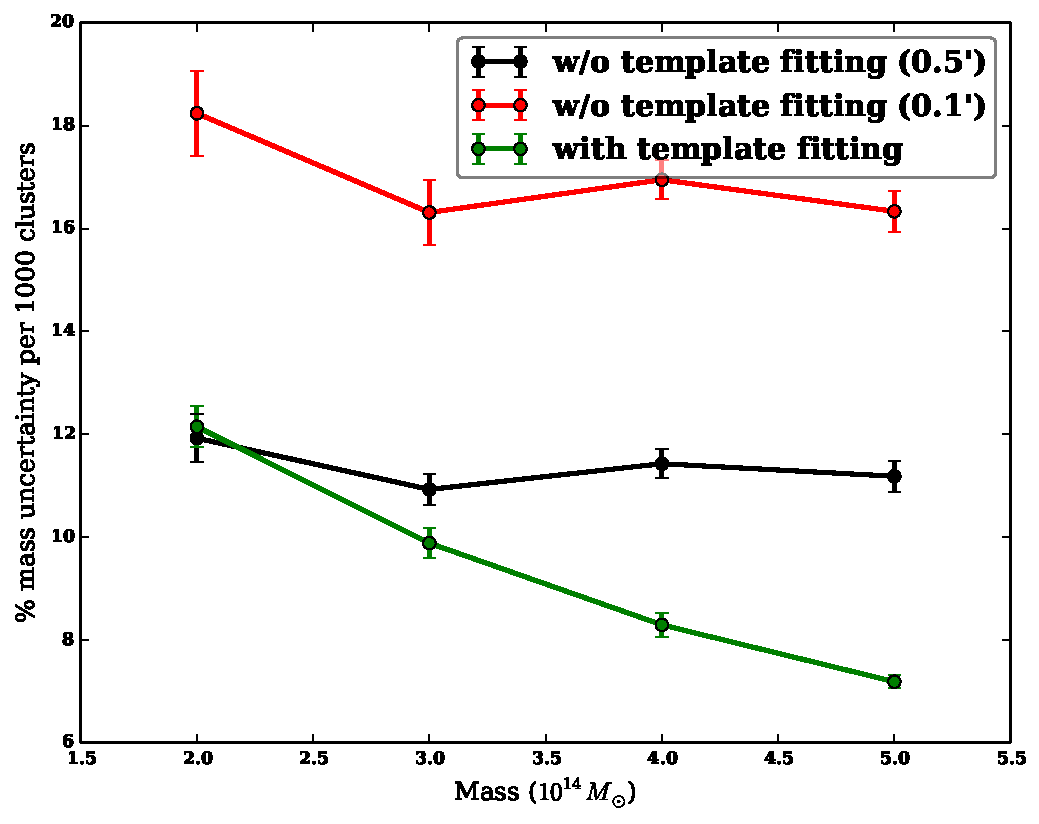
\includegraphics[width=\linewidth]{figs/miscentering_results.pdf}
 \caption{
Our new method is robust to realistic SZ simulations. 
The red and black solid curves show the performance of modified QE for the Sehgal and Takahashi simulations respectively. 
The dashed lines show the improvement in each case when template fitting is used to reduce the SZ variance in the lensing map. 
 \sr{ Change xlabel to $\mvir$}.
 }
\label{fig:realistic_sims}
\end{figure}

\section{Forecasts}
\label{forecasts}
Now we predict the uncertainties expected on the stacked mass for the cluster samples from the CMB-S4 \citep{cmbs4-sb1} and the Simons Observatory (SO)\footnote{\sr{SO Goal: write more}} \citep{SO18} experiments. 
In both cases, we only consider the large-aperture telescopes (LAT) with an experimental beam of $\theta_{\rm FWHM} = 1.^{\prime}4$ at 150 GHz and covering 40\% of the sky (see also Table \ref{table_forecast_setup}).
We generated the expected cluster samples for the experiments without any foreground reduction technique using the 150 GHz channel. 
For this, using simulations we first estimate the detection significance \snr{} for clusters as a function of mass and redshift for the two experiments. 
The simulations contain signals from the primordial CMB, Gaussian foregrounds uncorrelated with the cluster, cluster tSZ emission modelled using Arnaud profile, and the respective white noise levels as given in Table \ref{table_forecast_setup}.
The Gaussian foregrounds components were added using the measurements made by the SPT-SZ experiment \citep{george15} and contain emissions from radio, dusty galaxies, and the SZ signals from the low mass haloes that were unresolved by the SPT-SZ experiment. 
Next, we use the publicly available Halo Mass Function calculator \citep{murray13} to obtain the halo counts ($dN/dz/d{\rm log}M$) per unit redshift ($\Delta z = 0.1$) and mass ($\Delta M = xx$) bin. %https://arxiv.org/abs/1306.6721
Using the SNR look-up table from the above simulations, we get the number of clusters that will be detected above \snr$\ge 5$ by both the experiments. 
We estimate that CMB-S4 (SO) will detect approximately 75,000 (27,000) clusters.
More details about the software used tp generate the cluster sample will be given in a future work.
We feed these cluster samples into our lensing pipeline and predict the uncertainty in the stacked mass for the two samples. 
The results are given in Table \ref{table_forecast_setup}. 
\pending{ We find  ... w/o tSZ removal and xx after tSZ removal ..}
 \pending{bit about SO and S4 including configuration and improvements obtained }

\
}\fi





\iffalse{
\subsection{Modifying the Quadratic Estimator to remove SZ bias}
\label{sec_mQE}


Gravitational lensing by a compact object like a galaxy cluster creates a lensing dipole pattern in the direction of the large-scale CMB temperature gradient. 
The QE \citep{hu02a} is based on extracting the correlation between dipole and the background gradient to estimate the lensing convergence $\hat{\kappa}_{\bL}$. 
Specifically, the lensing convergence can be estimated from a weighted product of filtered versions of a gradient map $G(\hat{n})$ and  lensing lensing map $L(\hat{n})$: 
\begin{equation}
\hat{\kappa}_{\bL} = -A_{\ell} \int d^{2}\bnhat\ e^{-i\bnhat\cdot\bL}\ {\rm Re} \left\{ \nabla \cdot \left[ G(\bnhat) L^{*}(\bnhat)\right]\right\}.
\label{eq_QE_kappa}
\end{equation} 
Here, $\bnhat$ is the pointing unit vector, $\bL$ is angular multipole, and $A_{l}$ is a normalization factor. 


While designed to pull out the lensing-induced correlations between large-scale and lensing CMB anisotropy, the QE is also sensitive to  correlations due to foreground emission.
Of particular concern is  the cluster's own SZ emission, which is typically an order of magnitude larger than lensing signal. 
As shown by \citet{hu07}, the magnitude of the SZ bias can be lowered by decreasing the characteristic scale of the low pass filter on the gradient map. 
However, a stronger low-pass filter obviously reduces the number of modes used to measure the gradient, and thus decreases the signal-to-noise. 
The modified QE instead eliminates this bias by using an SZ-cleaned map for the large-scale gradient map. 
The large-scale gradient map is chosen because the CMB has much more power on large scales, so the noise penalty from SZ removal has minimal impact. 
Note that while multiple foregrounds can be removed in principle, in practice the focus has been on removing the SZ signal. 
This is simply because the SZ signal introduces the largest bias.  
With the SZ signal present in only one of the two maps, there is no SZ-induced correlation between the two maps and no net bias on the reconstruction of the lensing convergence. 
}\fi




\iffalse{
However the SZ emission in the small scale lensing map does add noise to the lensing reconstruction. 
Since under self-similarity the SZ flux, $y$, is expected to scale with  \mbox{cluster mass $M$} as $y \propto M^{5/3}$ while the lensing signal is linear in mass, the additional SZ variance will generally be more important for high-mass clusters. 
The SZ variance will also be more important in low-noise surveys, i.e.~when it is larger than the instrumental noise in the convergence map.%the nominal variance of convergence map set by the instrumental noise level of the experiment.  Cosmic Microwave Background (CMB) has no power at galaxy cluster angular scales due to silk damping and hence can be approximated as a gradient on arc minute scales.
 Gravitational lensing of CMB by cluster induces a dipole kind of structure on the top of gradient.
 The correlation between the background gradient and lensing dipole is known as gradient approximation.    
The QE \citep{hu02a} exploits the gradient approximation to estimate the lensing convergence profile $\hat{\kappa}$. 
 Gradient approximation doesn't hold for all Fourier modes, in fact it holds good for only those Fourier modes which are correlated by reconstruction. 
 Specifically, the lensing convergence can be estimated from a weighted product of filtered versions of a gradient map $G(\hat{n})$ and  lensing lensing map $L(\hat{n})$: 
\begin{equation}
\hat{\kappa}_{\bL} =-A_{\ell}\int d^{2}\bnhat\ e^{-i\bnhat\cdot\bL}\ {\rm Re} \left\{ \nabla \cdot \left[ G(\bnhat) L^{*}(\bnhat)\right]\right\}.
\label{eq_QE_kappa}
\end{equation} 
Here, $\bnhat$ is the pointing unit vector, $\bL$ is angular multipole, and $A_{l}$ is a normalization factor. 

While designed to pull out the lensing-induced correlations between large-scale and lensing CMB anisotropy, the QE is also sensitive to  correlations due to foreground emission.
Of particular concern is  the cluster's own SZ emission, which is typically an order of magnitude larger than lensing signal. 
Two ways have been discussed in literature to eliminate/reduce the SZ bias.
One way is to exploit the multiple frequency dependence of SZ signal and use linear combination of different frequencies to remove SZ.
While this method completes eliminates SZ bias, it significantly increases the statistical uncertainty due to the higher noise level of the combined map.
Another way is to lower the characteristic scale of the low pass filter on the gradient map as shown in  \citet{hu07}.
Lowering the gradient cut results in separation of the modes present in gradient and lensing dipole map; hence reducing the unwanted correlation. 
However, a stronger low-pass filter obviously reduces the number of modes used to measure the gradient, and thus decreases the signal-to-noise. 

On the other hand, the modified QE instead eliminates this bias without increasing the variance significantly by using an SZ-cleaned map for the large-scale gradient map. 
The large-scale gradient map is chosen because the CMB has much more power on large scales, so the noise penalty from SZ removal has minimal impact. 
Note that while multiple foregrounds can be removed in principle, in practice the focus has been on removing the SZ signal. 
This is simply because the SZ signal introduces the largest bias.  
With the SZ signal present in only one of the two maps, there is no SZ-induced correlation between the two maps and no net bias on the reconstruction of the lensing convergence. 

However the SZ emission in the lensing map does add noise to the lensing reconstruction. 
Since under self-similarity of the SZ flux, $y$, is expected to scale with cluster mass $M$ as $y\propto M^{5/3}$ while the lensing signal is linear in mass, the additional SZ variance will generally be more important for high-mass clusters. 
The SZ variance will also be more important in low-noise surveys, i.e.~when it is larger than the instrumental noise in the convergence map.%the nominal variance of convergence map set by the instrumental noise level of the experiment. 

\subsection{Template fitting to reduce the SZ variance}
\label{sec_sz_template_fitting}

As mentioned earlier, an obvious way to eliminate this SZ variance is by using SZ-free maps for both the lensing and gradient maps. 
Of course this would undo the advantages of the modified QE for the instrumental noise in the lensing map. 
One can also reduce this extra variance by projecting out a model template for the SZ signal, and thereby reducing the total amount of SZ power in the lensing map. 

Template fitting has been considered previously in the context of the original QE \citep{tbd?}. 
However, in that setting, residual SZ signals would bias the lensing masses. 
%\tbd{the next needs a citation/details on what size cluster} 
 Even one percent of residual SZ signal would lead to bias of six percent in mass estimation. 
This is not a problem in modified QE with SZ-free gradient map the residual SZ in the second leg won't introduce any bias. %within certain limits, template fitting and any residuals will not bias the modified QE.

To be unbiased, the template must not couple (on average) to the  CMB lensing signal. 
This can be achieved by either fitting the template to a Compton  y-map (i.e. using the different spectral dependence of the SZ and CMB to eliminate the CMB), or by using a template that has no average correlation with the lensing dipole pattern. 
The latter can be achieved by a radially symmetric template, fixed at the cluster position.
To illustrate this we constructed a plane temperature gradient field and lensed it with galaxy cluster of mass $M_{200m} = 5*10^{14}M_{\odot}$. 
We fit a radially symmetric Gaussian profile to the lensing dipole signal as shown in Fig. ~\ref{fig:no_bias}. 
 The left panel in Fig. ~\ref{fig:no_bias} is the lensing dipole signal and right panel is the best fit Gaussian profile. 
 As can be seen the amplitude of the resultant Gaussian fit is of the order of $10^{-15}$.

\begin{figure}
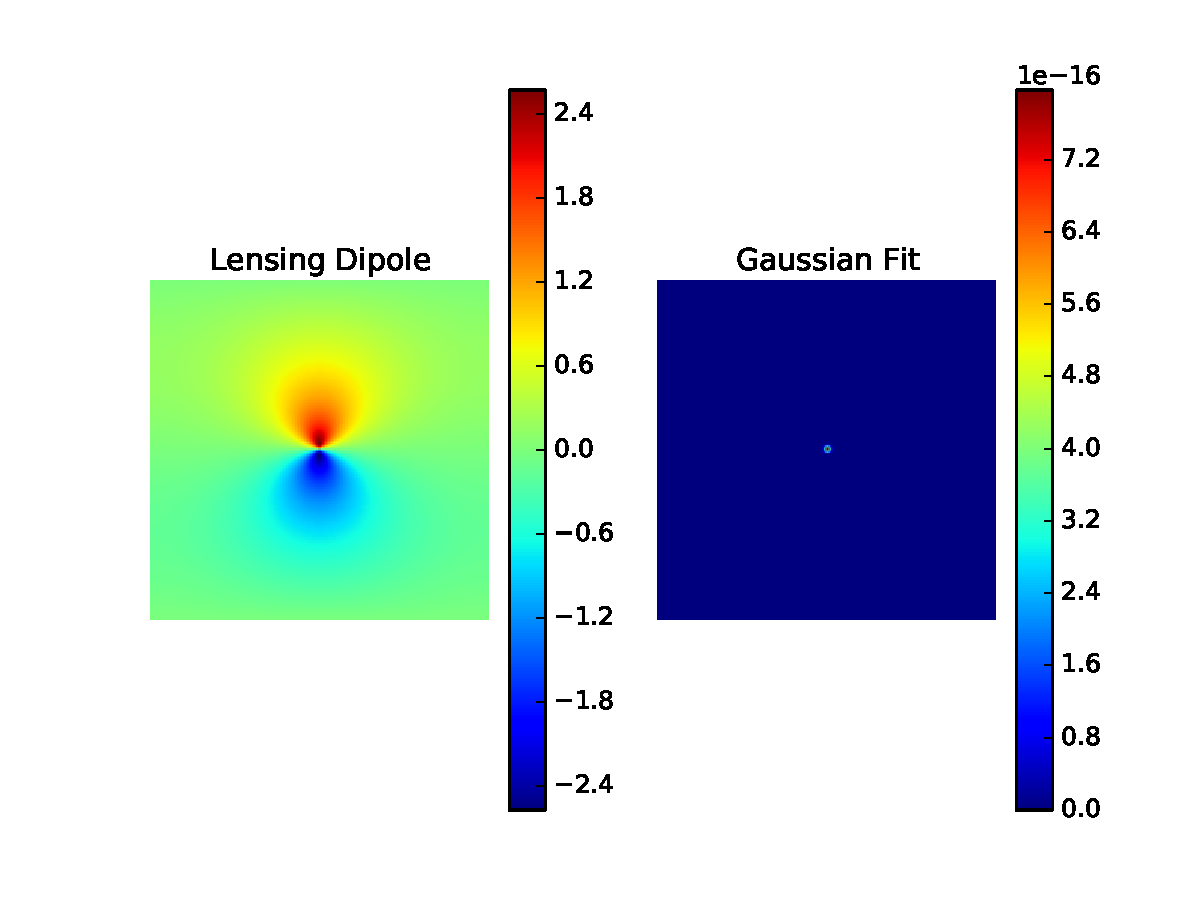
\includegraphics[width=\linewidth]{figs/template_fitting_bias.pdf}
 \caption{\pending{explain why no bias}
 } 
\label{fig:no_bias}
\end{figure}

If the position is freed, the template can shift to pick up the negative lobe of the lensing dipole signal resulting in a low bias. 
Given the impossibility in creating a `perfect' SZ template, the template fitting will not completely eliminate the SZ signal in the lensing map. 
However, template fitting can significantly reduce the SZ power in the lensing map, and thus reduce the SZ noise penalty on the lensing mass reconstruction. 

In this work, we take the tact of fitting a radially symmetric template at the fixed cluster location. 
Unless otherwise noted, we assume the beam to be a Gaussian with FWHM = 1\arcmin{} at 150 GHz and 1\arcmin.7 at 95\,GHz. 
As this beam size is significant compared to the actual size of clusters at $z>0.3$, clusters are approaching the effective point source limit where the specific details of their shape would not matter. 
Thus we choose to use a simple Gaussian template as the baseline template in this work. 
We also compare the results to template fitting with more physically motivated Arnaud profile \citep{arnaud10}, convolved by the experimental Gaussian beam.  
The residuals of removing a 2\arcmin.0 FWHM Gaussian from an Arnaud profile convolved by a 1\arcmin.7 beam are illustrated in Fig.~\ref{fig:residual}. 
As argued above, the Gaussian significantly reduces the SZ signal despite the mismatch between the assumed profile and input SZ model. 
While there should be small variations in the typical size of the cluster's SZ emission with mass and redshift, we neglect these variations and fix the size of the templates based on the expected median mass and redshift of the sample.

Since the template will be applied to that lensing map that has been high pass filtered at $\ell > 2000$, we apply a matching high pass filter to the map used for fitting and the SZ model template. 
This high-pass filter step is done in cutouts of $100\arcmin \times 100\arcmin$; we then pull out a central $10\arcmin \times 10\arcmin$ cutout at the cluster location for fitting the template. 
Since both the SZ emission and lensing signal extraction is concentrated within a few arcminutes of the cluster center, there is little reason to fit over a larger area. 
We allow for two free parameters in the fitting: the overall amplitude of the template, and a constant DC offset. 
Note that given the high-pass filter, we expect (and find) the DC term to be effectively zero. 
In any case, while we fit for a DC term when normalizing the template, we do not then remove the DC term. 
Only the template is subtracted from the lensing map.

With template fitting included, the Fourier transforms of the two maps used by the quadratic estimator can be written down as:
\begin{eqnarray}
G_{\ell} &=& i\ell W^{G}_{\ell} T^{\rm SZ-free}_{\ell}\\
L_{\ell} &=& W^{L}_{\ell} \left(T_{\ell} - T_\ell^{\rm SZ-template}\right)
\end{eqnarray}
where, $G_{\ell}$ is the large-scale gradient map and $L_{\ell}$ is the lensing map. 
$W^{G}_{l}$ and $W^{L}_{l} $ are the Wiener filters to maximize the lensing signal \cite{hu06}. 
The mm-wave map is $T_{\ell}$ while the constructed SZ-free map is $T^{\rm SZ-free}_{\ell}$. 
Compared to the modified QE \citep{madhavacheril15,raghunathan18}, the new element is the $T_\ell^{\rm SZ-template}$ term representing the SZ template fit. 

\begin{figure}
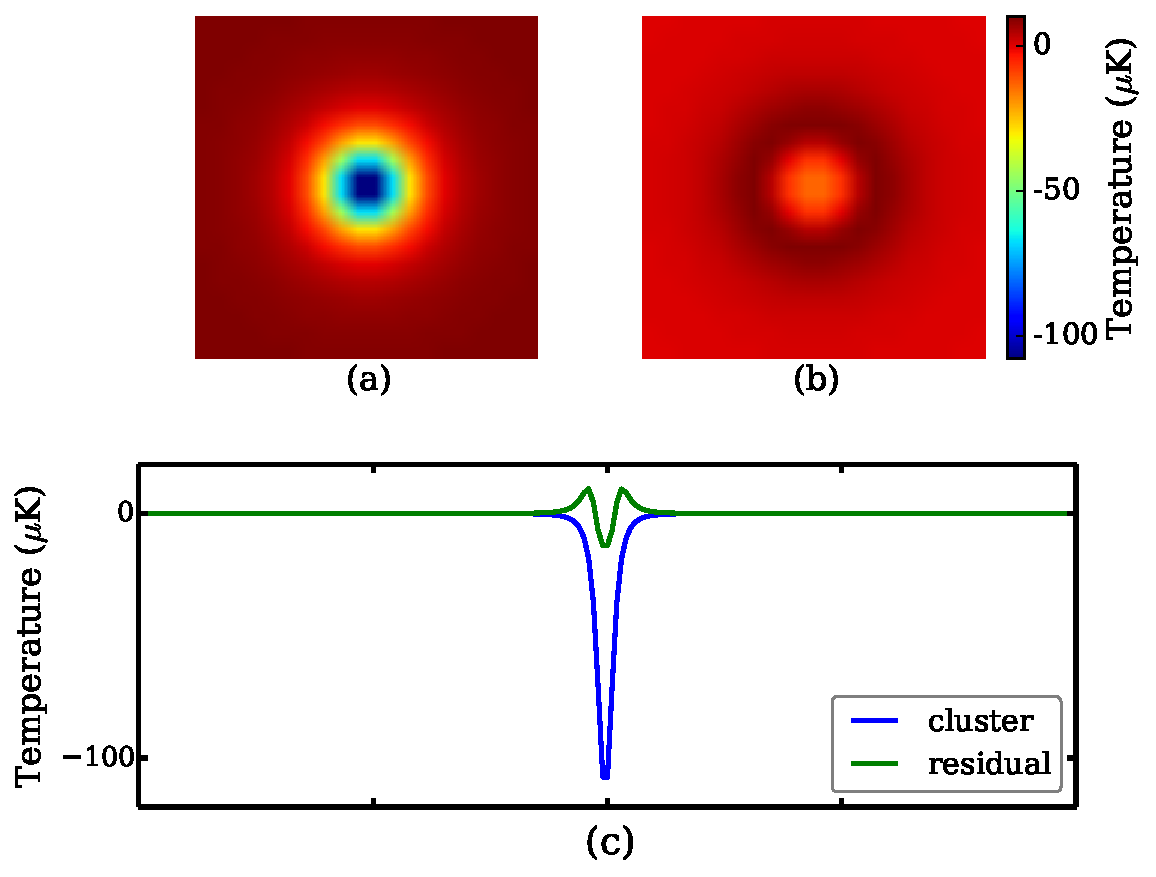
\includegraphics[width=\linewidth]{figs/template_fitting.pdf}
 \caption{Template fitting significantly reduces SZ power, even with an imperfect match between the template and true SZ signal. 
The top left panel (a) shows the expected Arnaud profile for a galaxy cluster of mass zzjksfsjk$\mvir = 5 \times \: 10^{14}M_{\odot}$ at z=0.7 after being smoothed by Gaussian beam with FWHM= 1\arcmin.7.
The top right panel (b) shows the residuals after subtracting the best-fit 2\arcmin.0 FWHM Gaussian (the amplitude is free, but the FWHM is fixed). 
The lower panel (c) shows one-dimensional slices through each panel: the solid, blue line is a slice through the beam-convolved Arnaud profile of (a), and the dashed green line is a slice through the residual map in (b). 
 } 
\label{fig:residual}
\end{figure}
}\fi